% flashcards-title: Two measurement results as uncertainty bars on one number line
% flashcards-desc: A number line of lengths in centimeters runs from twelve to thirteen with labeled marks every two tenths and small steps at every tenth. Above it sit two results, one over the other. Each result is drawn as a filled dot at its best value with a horizontal bar through the dot spanning its uncertainty interval, the bar ends marked by short vertical caps. The lower bar is labeled A, twelve point four plus or minus zero point one centimeters; the upper bar is labeled B, twelve point six plus or minus zero point two centimeters. Whether the two bars share any stretch of the scale is left to the reader.
\documentclass[dvisvgm,tikz,border=8pt]{standalone}
\usepackage{tikz}
\usetikzlibrary{arrows.meta,calc,positioning}
\definecolor{DeckInk}{HTML}{172A3A}
\definecolor{DeckAccent}{HTML}{176B87}
\definecolor{DeckWarm}{HTML}{D97706}
\definecolor{DeckMuted}{HTML}{667784}
\definecolor{DeckPaper}{HTML}{F7FAFC}
\tikzset{
  every node/.style={font=\sffamily, text=DeckInk},
  object/.style={draw=DeckInk, line width=1.1pt, fill=DeckPaper},
  primary/.style={draw=DeckAccent, line width=1.5pt},
  boundary/.style={draw=DeckAccent, line width=1.5pt, dashed, rounded corners=6pt},
  guide/.style={draw=DeckMuted, line width=0.9pt, dashed},
  dimension/.style={{Stealth[length=3.2mm,width=2.2mm]}-{Stealth[length=3.2mm,width=2.2mm]}, draw=DeckWarm, line width=1.2pt},
  motion/.style={-{Stealth[length=3.5mm,width=2.5mm]}, draw=DeckAccent, line width=1.5pt, dashed},
}

\begin{document}
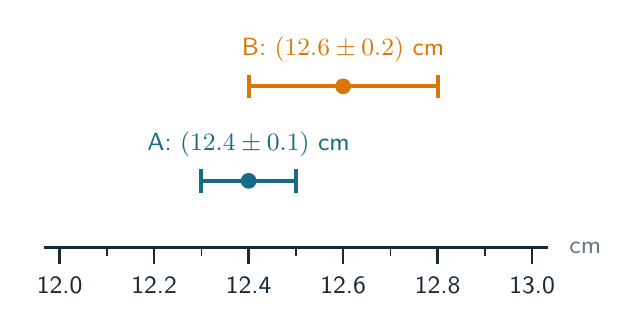
\begin{tikzpicture}[x=1cm,y=1cm]
  % Axis: x = (value - 12.0) * 6
  \draw[DeckInk, line width=1.1pt] (-0.2,0) -- (6.2,0);
  \foreach \x in {0,0.6,...,6.0}
    \draw[DeckInk, line width=0.5pt] (\x,0) -- (\x,-0.1);
  \foreach \x/\v in {0/12.0, 1.2/12.2, 2.4/12.4, 3.6/12.6, 4.8/12.8, 6.0/13.0}{
    \draw[DeckInk, line width=0.9pt] (\x,0) -- (\x,-0.2);
    \node[font=\sffamily\small] at (\x,-0.48) {\v};
  }
  \node[font=\sffamily\small, text=DeckMuted, anchor=west] at (6.35,0) {cm};
  % Result A: 12.3 to 12.5, best value 12.4
  \draw[DeckAccent, line width=1.5pt] (1.8,0.85) -- (3.0,0.85);
  \draw[DeckAccent, line width=1.5pt] (1.8,0.7) -- (1.8,1.0);
  \draw[DeckAccent, line width=1.5pt] (3.0,0.7) -- (3.0,1.0);
  \fill[DeckAccent] (2.4,0.85) circle (0.1);
  \node[font=\sffamily\small, text=DeckAccent] at (2.4,1.32) {A: $(12.4 \pm 0.1)$ cm};
  % Result B: 12.4 to 12.8, best value 12.6
  \draw[DeckWarm, line width=1.5pt] (2.4,2.05) -- (4.8,2.05);
  \draw[DeckWarm, line width=1.5pt] (2.4,1.9) -- (2.4,2.2);
  \draw[DeckWarm, line width=1.5pt] (4.8,1.9) -- (4.8,2.2);
  \fill[DeckWarm] (3.6,2.05) circle (0.1);
  \node[font=\sffamily\small, text=DeckWarm] at (3.6,2.52) {B: $(12.6 \pm 0.2)$ cm};
\end{tikzpicture}
\end{document}
